\chapter*{Практика 4. QPSK модуляция}
\addcontentsline{toc}{chapter}{Практика 4. QPSK модуляция}
\label{ch:4_practice}

\textit{\textbf{Задание:}} Реализовать QPSK модулятор.

\begin{itemize}
    \item Реализован QPSK маппер для отображения пар бит в комплексные символы:
    \begin{itemize}
        \item (0,0) $\rightarrow$ $0.707 + 0.707i$
        \item (0,1) $\rightarrow$ $0.707 - 0.707i$
        \item (1,0) $\rightarrow$ $-0.707 + 0.707i$
        \item (1,1) $\rightarrow$ $-0.707 - 0.707i$
    \end{itemize}
    \item Проведена проверка корректности модуляции
\end{itemize}

\begin{figure}[ht]
    \centering
    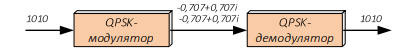
\includegraphics[width=0.8\textwidth]{qpsk_mapping.png}
    \caption{QPSK отображение битовых пар в символы}
    \label{fig:qpsk_mapping}
\end{figure}

\begin{figure}[ht]
    \centering
    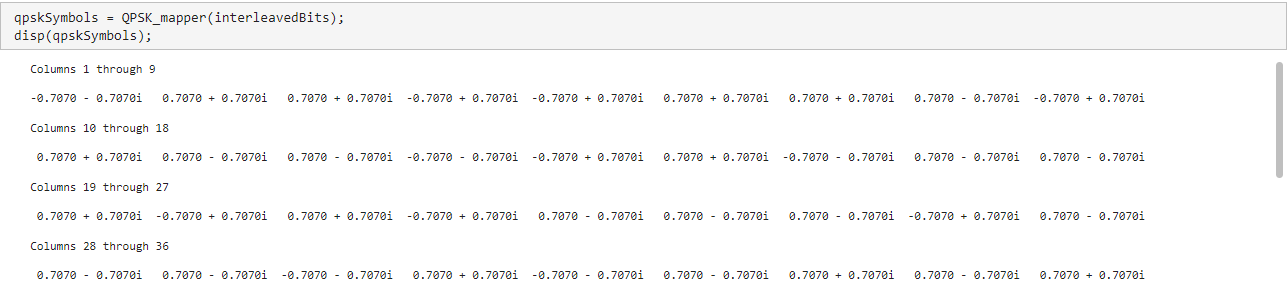
\includegraphics[width=0.8\textwidth]{4practice_result.png}
    \caption{Результат четвёртой практики}
    \label{fig:4practice_result}
\end{figure}